\documentclass{article}
\usepackage{graphicx} % Required for inserting images
\usepackage{listings}
\usepackage{xcolor} % for coloring code keywords

\title{ Model Quantization}
\author{Maya Sharaf}
\date{July 2026}


%customize the code section
\lstset{
    language=Python,                % Choose the default language
    basicstyle=\ttfamily\small,     % Code font and size
    keywordstyle=\color{blue},      % Color for keywords
    stringstyle=\color{darkgray},   % Color for strings
    commentstyle=\color{gray},      % Color for comments
    numbers=left,                   % Position of line numbers
    numberstyle=\tiny\color{gray},  % Style of line numbers
    stepnumber=1,                   % Number every line
    breaklines=true,                % Wrap long lines automatically
    frame=single                    % Add a box frame around the code
}

\begin{document}

\maketitle

\section{Introduction}
\normalsize {
Most modern large-scale Transformer-based models (BERT, LLaMA, etc.) typically contain hundreds of millions up to tens of billions of parameters in the form of 32-bit floating-point numbers.

That causes big VRAM/RAM consumption, high latency, and energy consumption,  making it impossible to deploy these models on smaller devices.}

\section{What quantization does}

\normalsize { Quantization refers to mapping high-precision numbers such as float32 weights to a lower precision representation using few bits such as int8 or int4.

For example, moving from 32-bit to 8-bit representation leads to reduction in memory footprint by approximately 4× and faster inference if the underlying hardware is capable of efficiently executing integer operations.
}

\begin{figure}[htbp]
    \centering % Centers the image horizontally
    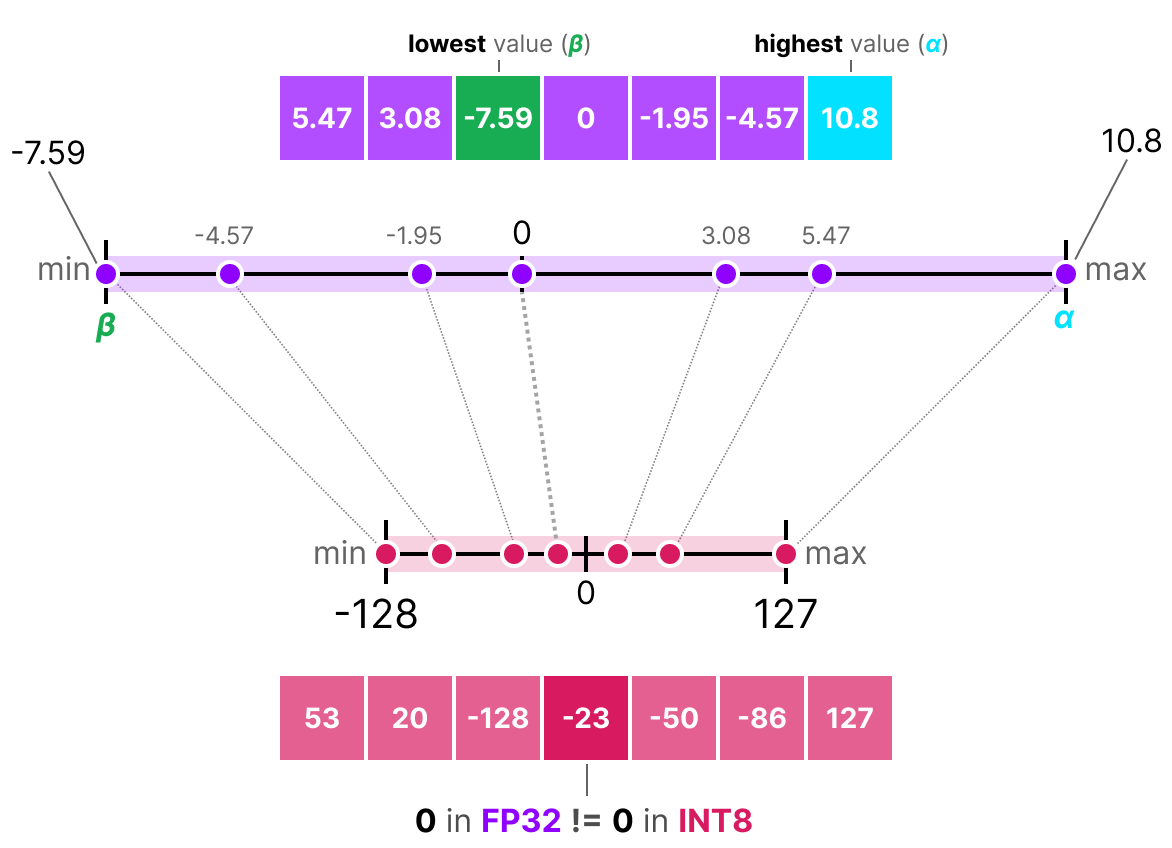
\includegraphics[width=0.7\textwidth]{quantization}
    \caption{Scaling diagram}
    \label{fig:scaling}
\end{figure}

\normalsize {
The idea is that one chooses a range like 
[xmin,xmax]
and scales it linearly to an integer range such as [-128,127] for int8 as seen in Figure \ref{fig:scaling}
,then one saves the integer number along with scale/offset.
During inference, you dequantize back to approximate the original float values.}

\section{Quantization Techniques}

\subsection{Post‑Training Quantization (PTQ)}
\normalsize { 
Quantize a pretrained model without (or with minimal) retraining.
Simple and fast; often used for LLMs with calibration data.}

\subsection{Quantization‑Aware Training (QAT)}

\normalsize { 
Simulate quantization effects during training so the model learns to be robust to rounding and clipping.
Gives better accuracy but requires retraining.}

\subsection{Dynamic quantization}

\normalsize { 
Weights are quantized ahead of time; activations are quantized on the fly at runtime.
Very easy to use in frameworks like PyTorch and works well for Transformer layers.}


\subsection{Static quantization}

\normalsize { 
Both weights and activations are quantized using ranges estimated from a calibration dataset.
Can give better speed/size benefits but needs more engineering.

}



\paragraph{
For very large LLMs (LLaMA, etc.), you also see “weight‑only” schemes (only weights quantized, activations kept in fp16) and advanced methods like GPTQ, AWQ, SmoothQuant, etc.}



\section{Benefits and trade‑offs}

\subsection{Benefits:}

\begin{itemize}
    \item 4× memory reduction when going from fp32 to int8 for weights.
    \item Potential latency speedups when integer kernels are optimized on the target hardware.
    \item Enables serving larger models on smaller GPUs/CPUs or even edge devices.
\end{itemize} 

\subsection{Trade‑offs:}

\begin{itemize}
    \item Some accuracy/perplexity degradation, more noticeable at very low bit‑width (4‑bit and below).
    \item Quantization can be more complex for attention layers and outlier activations, so advanced schemes are often needed for large LLMs.
    \item Hardware support and library maturity determine the actual speed gains.
\end{itemize} 


\section{Code Example: 8‑bit / 4‑bit DistillBert with bitsandbytes (Hugging Face)}

\normalsize{For LLama‑style LLMs, weight‑only 8‑bit or 4‑bit quantization via bitsandbytes and Hugging Face transformers is common.
This lets you load multi‑billion‑parameter models on a single consumer GPU.}

\begin{lstlisting}[caption={Finetuning DistillBERT with LoRA}, label={code:python_quantize}]
from transformers import AutoModelForCausalLM, AutoTokenizer, BitsAndBytesConfig
import torch

model_name = "meta-llama/Llama-2-7b-hf"  # example; requires proper access

# 1. Configure 4-bit quantization (NF4) with bitsandbytes
bnb_config = BitsAndBytesConfig(
    load_in_4bit=True,                # or load_in_8bit=True for 8-bit
    bnb_4bit_compute_dtype=torch.float16,
    bnb_4bit_use_double_quant=True,   # nested quantization for better compression
    bnb_4bit_quant_type="nf4"         # "nf4" often works better than pure int4
)

# 2. Load tokenizer
tokenizer = AutoTokenizer.from_pretrained(model_name)

# 3. Load model directly in 4-bit on GPU
model = AutoModelForCausalLM.from_pretrained(
    model_name,
    quantization_config=bnb_config,
    device_map="auto"  # spreads layers across available devices if needed
)

# 4. Test generation
prompt = "Quantization enables large language models to run on smaller devices because"
inputs = tokenizer(prompt, return_tensors="pt").to(model.device)

with torch.no_grad():
    generated = model.generate(
        **inputs,
        max_new_tokens=50,
        do_sample=True,
        temperature=0.7
    )

print(tokenizer.decode(generated[0], skip_special_tokens=True))

\end{lstlisting}

\normalsize{The model weights are loaded directly in 4‑bit form, drastically reducing VRAM usage.
Computation uses fp16 activations with int4 weights, so you get a strong memory reduction with relatively small accuracy loss.
}

\end{document}
